\begin{figure}
\begin{center}
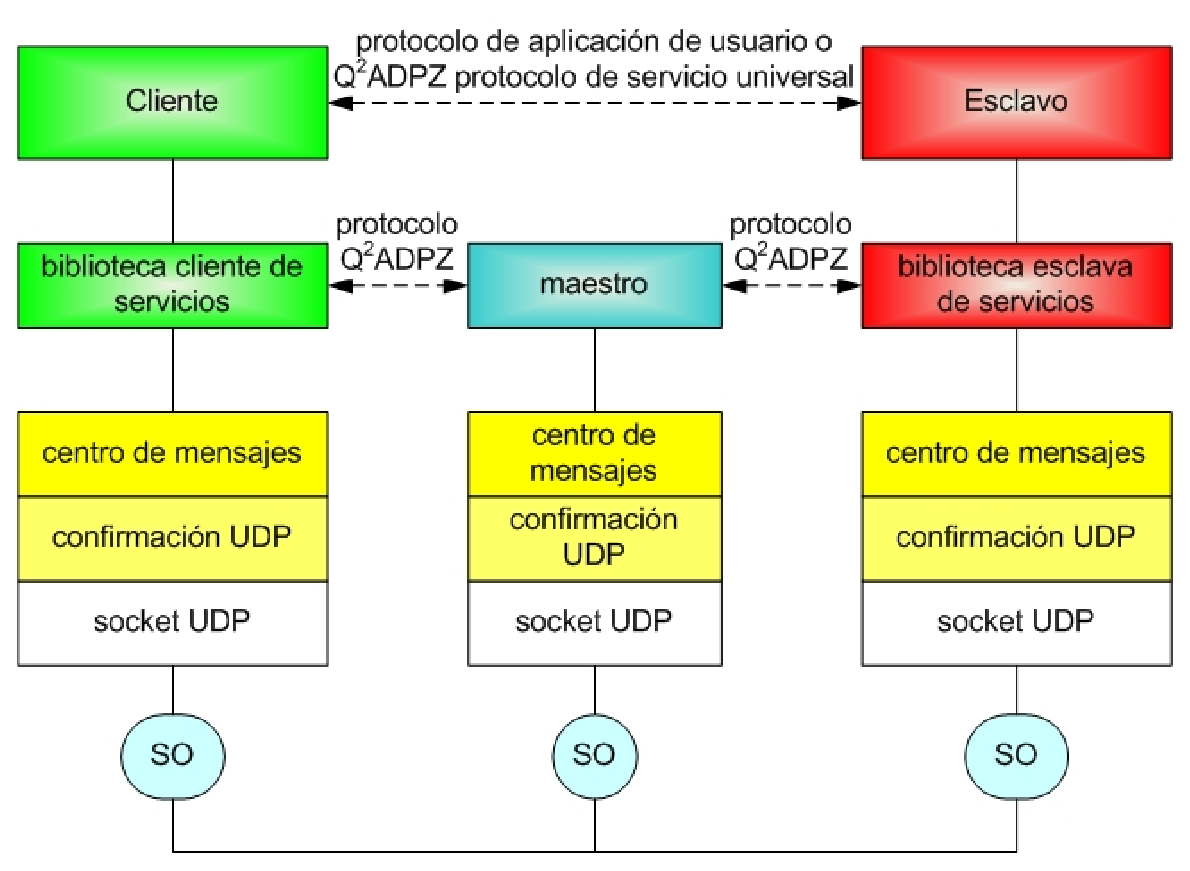
\includegraphics[width=0.7\textwidth]{images/image02.eps}
\end{center}
\caption{Las capas de comunicaci�n de Q$^2$ADPZ}
\label{fig:image02}
\end{figure}
La comunicaci�n en Q$^{2}$ADPZ est� basada en UDP, un protocolo de comunicaci�n poco fiable, en donde no est� garantizado que los paquetes enviados lleguen a su destino y si lo hacen, puede que no lleguen en el orden correcto. La ventaja de UDP sobre su alternativa, TCP, es su rapidez gracias a que carece de m�ltiples mecanismos enfocados en la conexi�n que implican una carga adicional a la comunicaci�n. Esta base conforma la primera capa de abstracci�n llamada \emph{socket UDP} que tiene como prop�sito la transmisi�n de mensajes de control usados dentro del sistema. Sobre esta base de comunicaci�n UDP, existe una capa superior de abstracci�n llamada \emph{confirmaci�n UDP}. El prop�sito de esta capa es darle m�s fiabilidad a UDP mediante mensajes de confirmaci�n para los mensajes enviados.

La siguiente capa es el \emph{centro de mensajes} que recibe y env�a mensajes de alto nivel - elementos XML. Estos mensajes son intercambiados en formato XML de acuerdo al protocolo definido para las comunicaciones cliente-maestro y maestro-esclavo. Esta capa es s�lamente utilizada para prop�sitos de control de las entidades del sistema. Para transferir los archivos necesarios para la ejecuci�n de tareas se utiliza el protocolo HTTP.  La figura \ref{fig:image02} grafica el modelo de comunicaci�n antes descrito.